\chapter{Ingénierie des exigences}
\section{Approche Top-Down}
\vspace{1.5cm}
Dans cette partie nous allons analyser notre système avec une approche Top-Down. Cela signifie que nous adopterons une démarche de conception descendante. Pour cela nous avons tracé le diagramme "bête à cornes", que l'on peut voir sur la figure \ref{fig:beteacorne}. Il permet de représenter graphiquement l'expression du besoin. Comme on peut le voir sur le diagramme, le système BMONS rend service aux apiculteurs en agissant sur une ou plusieurs ruches. Il a pour but d'aider la surveillance d'un rucher et d'avertir l'apiculteur en cas de problème.


\begin{figure}[h!]
\centering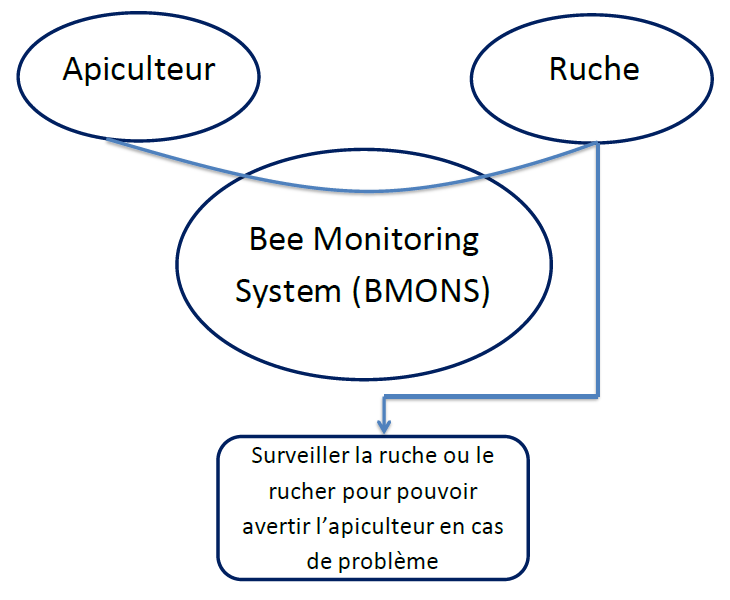
\includegraphics[scale=0.5]{BeteACornesBMONS.png}
\caption{\label{fig:beteacorne} Diagramme "bête à cornes" du système BMONS}
\end{figure}

Le diagramme pieuvre, \ref{fig:diagpieuvre1} et \ref{fig:diagpieuvre2}, nous permet ensuite de faire apparaître les fonctions principales du système. On peut aussi y retrouver les fonctions de services et de contraintes.

 
\begin{figure}[h!]
\centering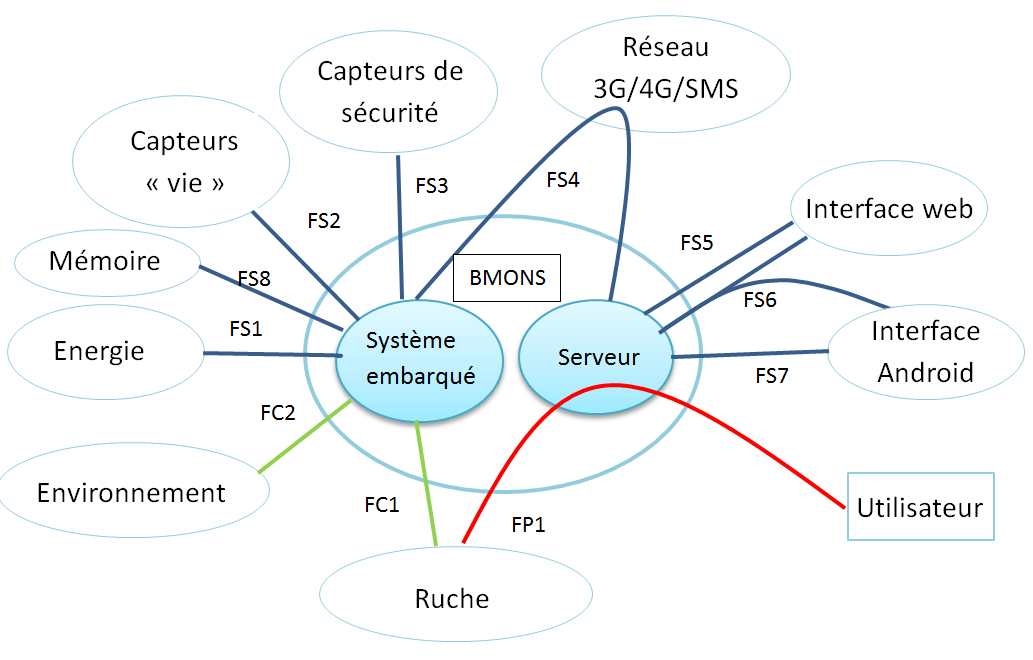
\includegraphics[scale=0.6]{pieuvre1.png}
\caption{\label{fig:diagpieuvre1} Diagramme pieuvre du système BMONS}
\end{figure}

\begin{figure}[h!]
\centering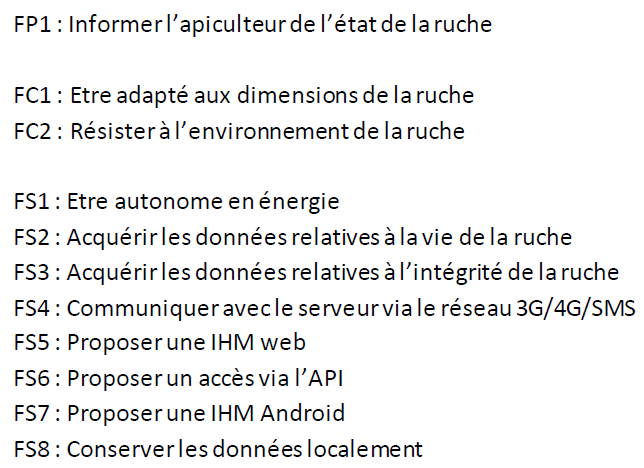
\includegraphics[trim = 1cm 0.5cm 13cm 1cm,scale=0.6]{pieuvre2.png}
\caption{\label{fig:diagpieuvre2} Légende diagramme pieuvre du système BMONS}
\end{figure}

\clearpage

\section{Approche Bottom-Up}

\vspace{1.5cm}
Nous allons maintenant adopter la démarche inverse, mais néanmoins complémentaire, de l'approche Top-Down. Il s'agit de l'approche Bottom-Up. C'est une démarche de conception ascendante qui va nous permettre d'avoir une vision plus globale du système. On peut voir sur \ref{fig:exi1} et \ref{fig:exi2} les exigences issues de cette analyse.

 
\begin{figure}[h!]
\centering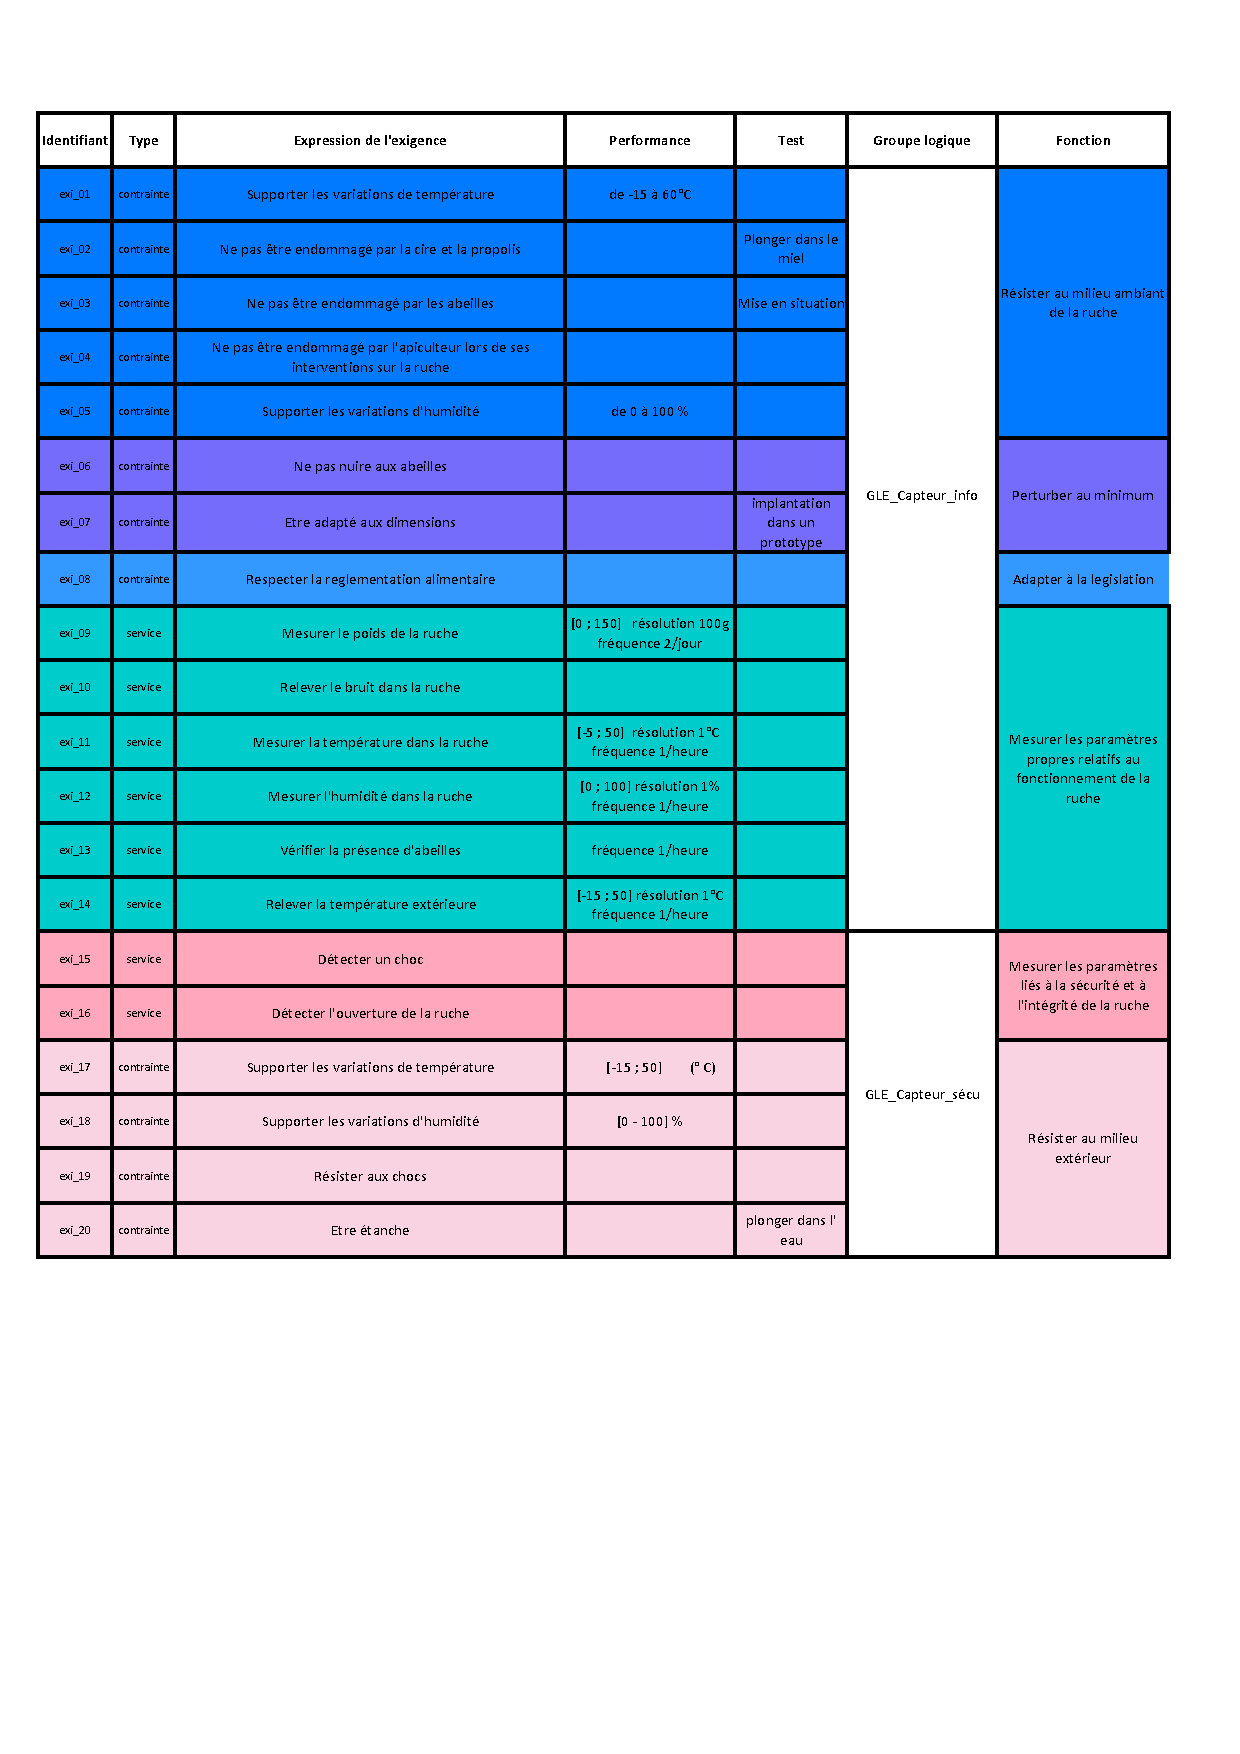
\includegraphics[trim = 1cm 8.7cm 1cm 1cm,scale=0.8]{Exigences_du_Projet_1.pdf}
\caption{\label{fig:exi1} Exigences issues de l'approche Bottom-Up (1/2)}
\end{figure}

 
\begin{figure}[h!]
\centering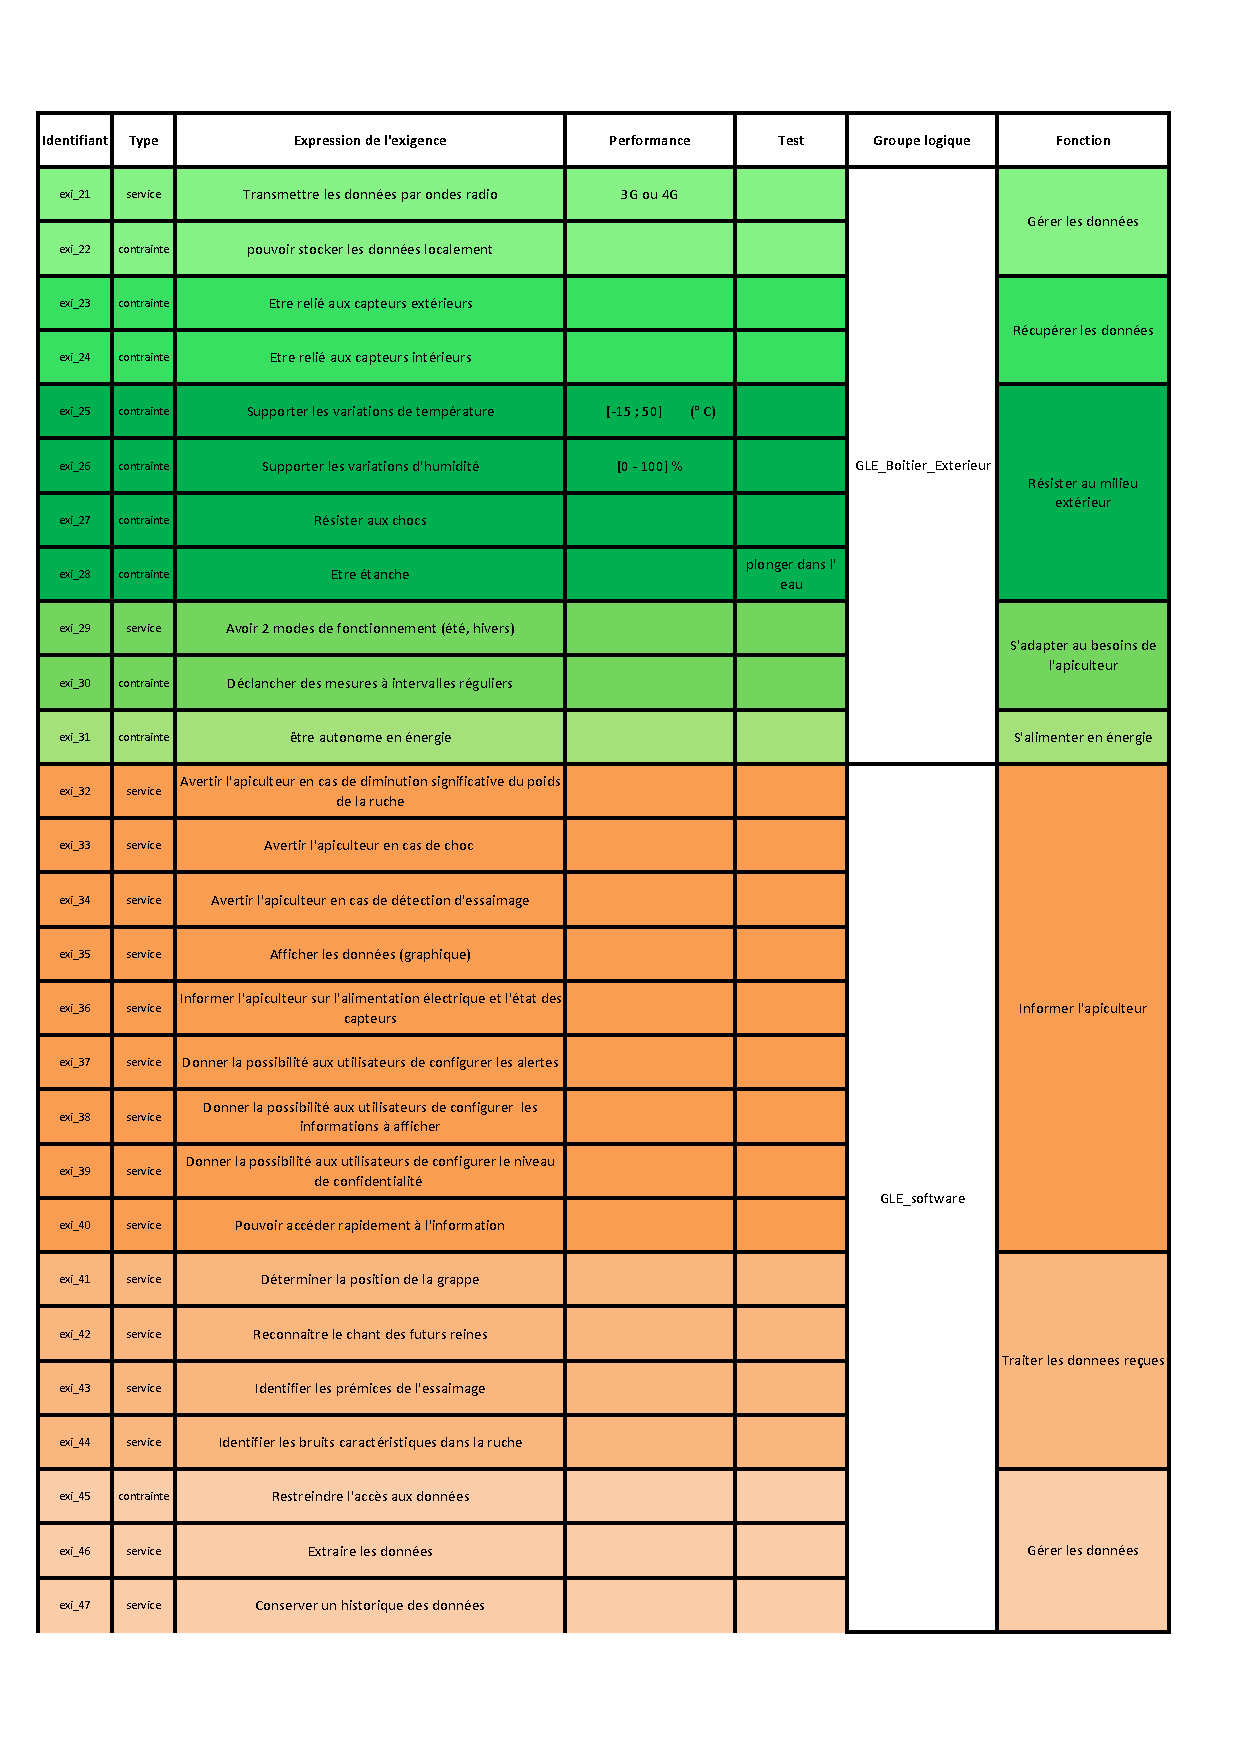
\includegraphics[trim = 1cm 2cm 1cm 1cm,scale=0.8]{Exigences_du_Projet_2.pdf}
\caption{\label{fig:exi2} Exigences issues de l'approche Bottom-Up (2/2)}
\end{figure}

\clearpage

\section{Fonctions métiers du système}
\vspace{1.5cm}

Après avoir réalisé une approche du point de vue "concepteur" du système, nous allons maintenant nous intéresser à la formulation des fonctions qu'un apiculteur souhaiterai avoir pour pouvoir suivre l'évolution de son rucher. Ces fonctions métiers ont été discutées avec notre client, monsieur Singhoff. Elles sont représentées sur les figures \ref{fig:exi1,exi2,exi3,exi4} en annexe dont la figure \ref{fig:exi1text} est un extrait.


\begin{figure}[h!]
\centering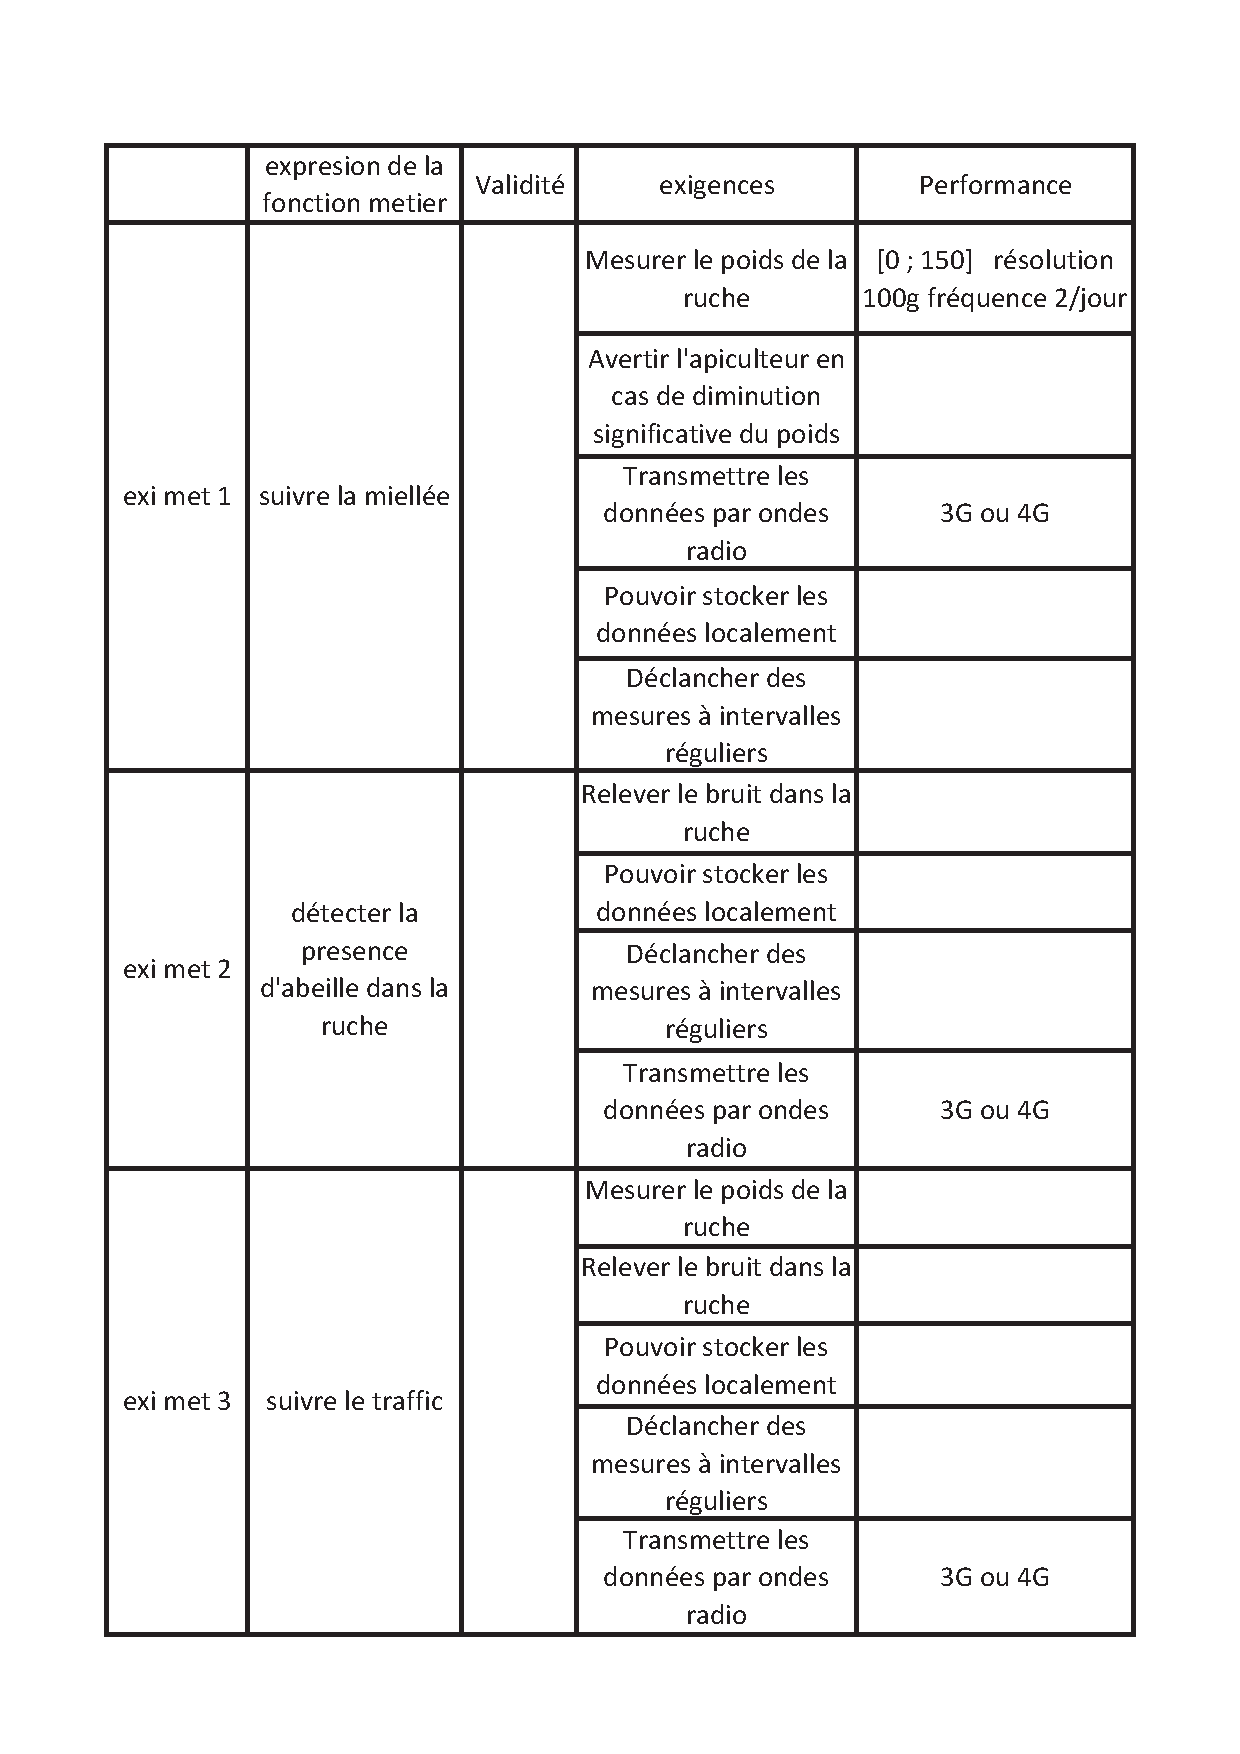
\includegraphics[trim = 1cm 2cm 1cm 1cm,scale=0.65]{Exigences1.pdf}
\caption{\label{fig:exi1text} Fonctions métiers du système (1/4)}
\end{figure}



\clearpage


\chapter{Architecture fonctionnelle}

L'étude de la spécification fonctionnelle trois axes a permis d'établir l'architecture fonctionnelle du système qui est représentée sur la figure \ref{fig:anaFonc}.
Ce schéma résume les interactions entre chaque partie: Bee Monitor qui regroupe l'ensemble des capteurs, la carte Arduino ainsi que la carte SSD pour l'enregistrement local des données, le module de transmission et le système d'alimentation rendant notre projet autonome en énergie et le serveur. Chaque acteur interagissant avec le système est également représenté: Les abeilles/ruche, l'apiculteur et l'environnement.   
  

\begin{figure}[h]
\centering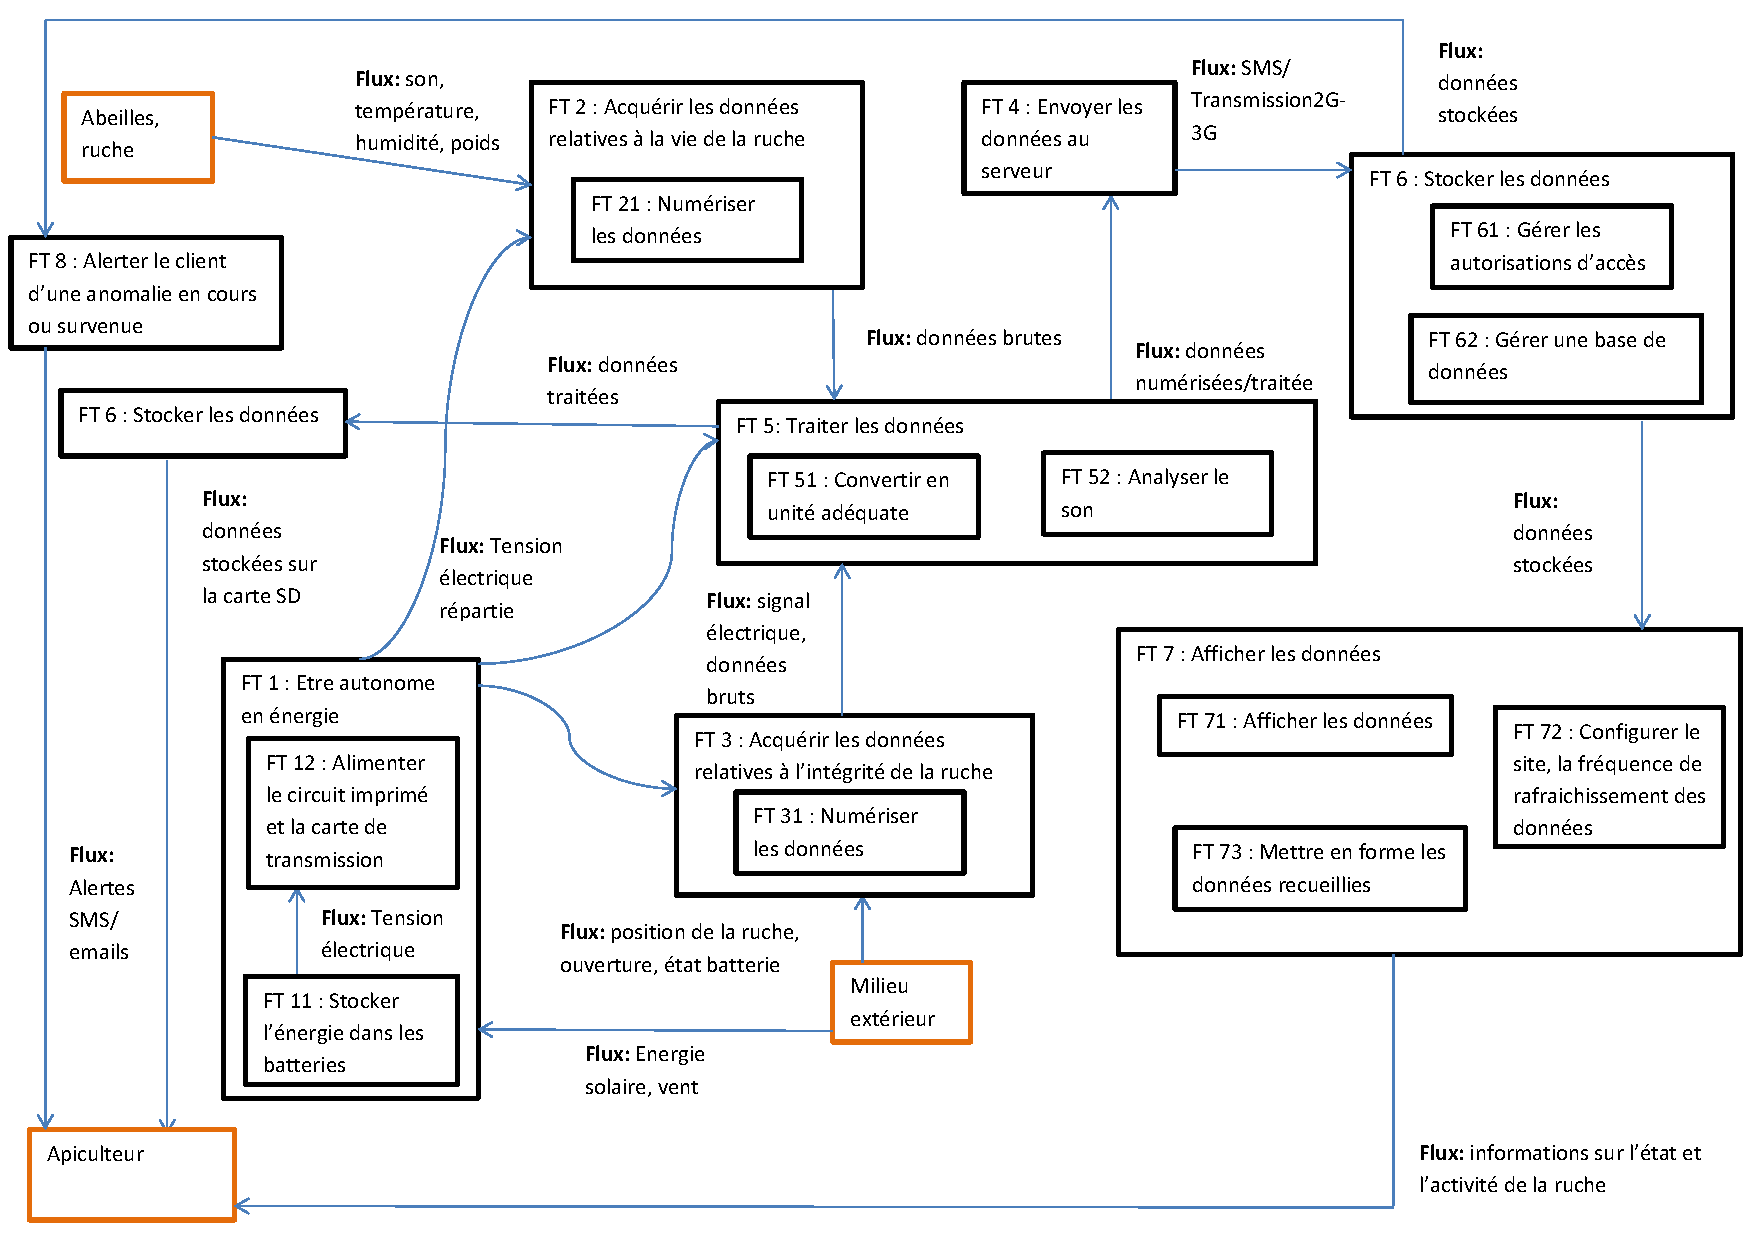
\includegraphics[scale=0.5]{analyseFonctionelle1.pdf}
\caption{\label{fig:anaFonc} Architecture fonctionnelle}
\end{figure}    

